
% ################################# Paragraph #################################
% Short introduction into the cataylsis section
In the following section we will demonstrate the merit of our bulk crystal searching method by investigating the 4 most stable structures for the oxygen evolution reaction, an important electrochemical reaction with application in energy storage technologies.


% | - Bulk Pourbaix
\subsubsection{Bulk Pourbaix}

% ################################# Paragraph #################################
% COMBAK
The electrochemical stability phase diagram (E vs. pH) was constructed from all bulk crystals of Ir, \ce{IrO_2}, \ce{IrO_3}, and aqueous dissolved \ce{IrO[4-]}.
Only the most stable structure for each stoichiometry is visible on the Pourbaix diagram which correspond to TEMP and are shown in Fig. \ref{fig:bulk_pourbaix}
% COMBAK Reference 4 most stable structres from elsewhere
% Also explain the Ir and IrO[4-] ion

% ################################# Paragraph #################################
Under acidic condition (< pH 7) and in the bias region of of interest for the OER, there exists a region of stability for the novel $\alpha$-AlF3 IrO3 structure found herein.

% ################################# Paragraph #################################
% COMBAK Insert bound of stability here
At a pH=0 the bound of stability for $\alpha$-AlF3 IrO3 spans TEMP

% | - Figure | Bulk Pourbaix Diagram
\begin{figure}
\centering
\makebox[\textwidth][c]{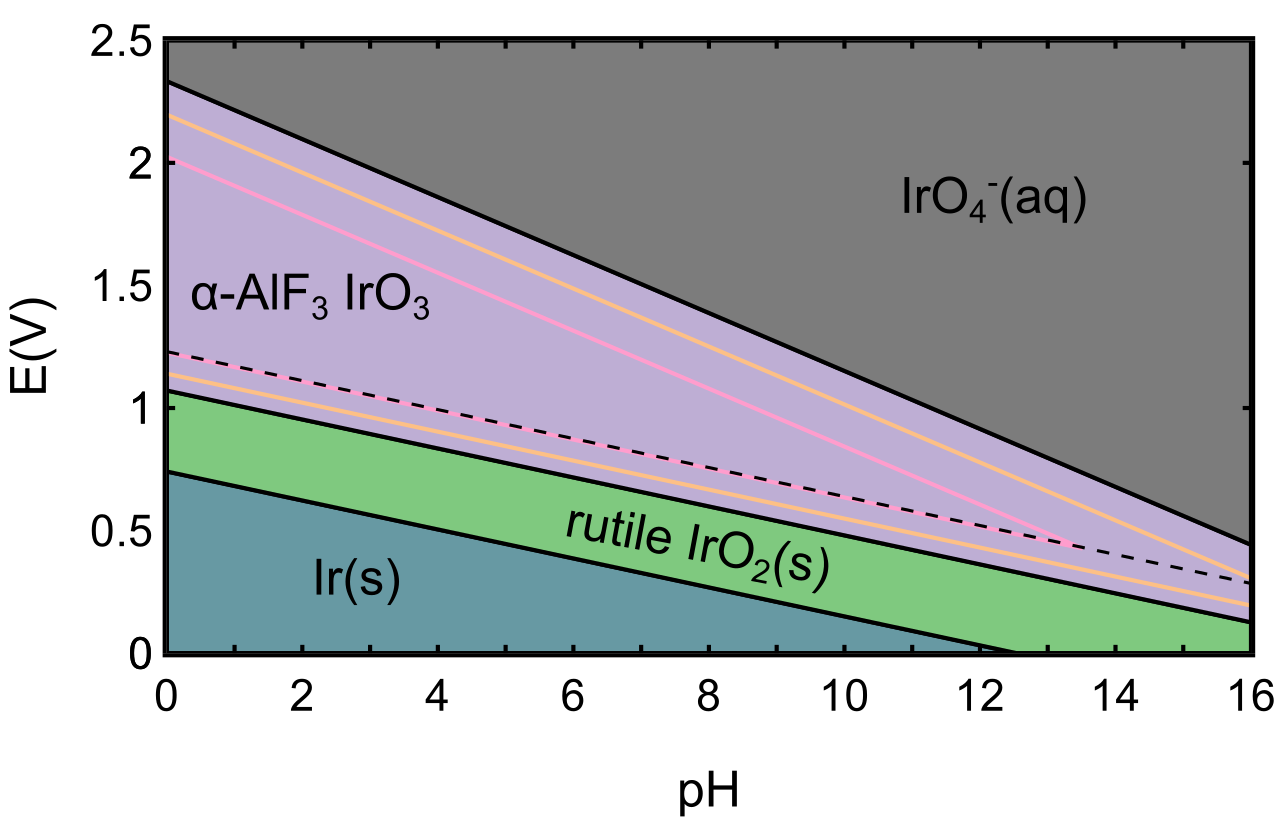
\includegraphics
{02_figures/oer_activity_stability/00_master__bulk-pourbaix__v1__400dpi__0__outplot.png}
% {02_figures/oer_activity_stability/bulk_pourbaix_0.pdf}
}
\caption{\label{fig:bulk_pourbaix}
Electrochemical bulk phase stability diagram (Pourbaix) of the Ir-O-H chemical space.
}
\end{figure}
% __|

% __|

% | - OER Activities and Surfaces
\subsubsection{b. OER Activities and Surfaces}

% ################################# Paragraph #################################
% Surface Energy Pourbaix Analysis

The OER activity (expressed in over-potential) for surfaces cut from the IrO2, and the 3 most stable polymorphs of IrO3 are shown in Fig. \ref{fig:oer_volcano}.
% TODO #reference | Reference for VESTA x-ray diff. pattern method
The specific facets were chosen from the highest intensity x-ray diffraction peaks from powder-diffraction spectra simulated in VESTA.


% | - Figure | OER Volcano/Surface Pourbaix
\begin{figure}
\centering
\makebox[\textwidth][c]{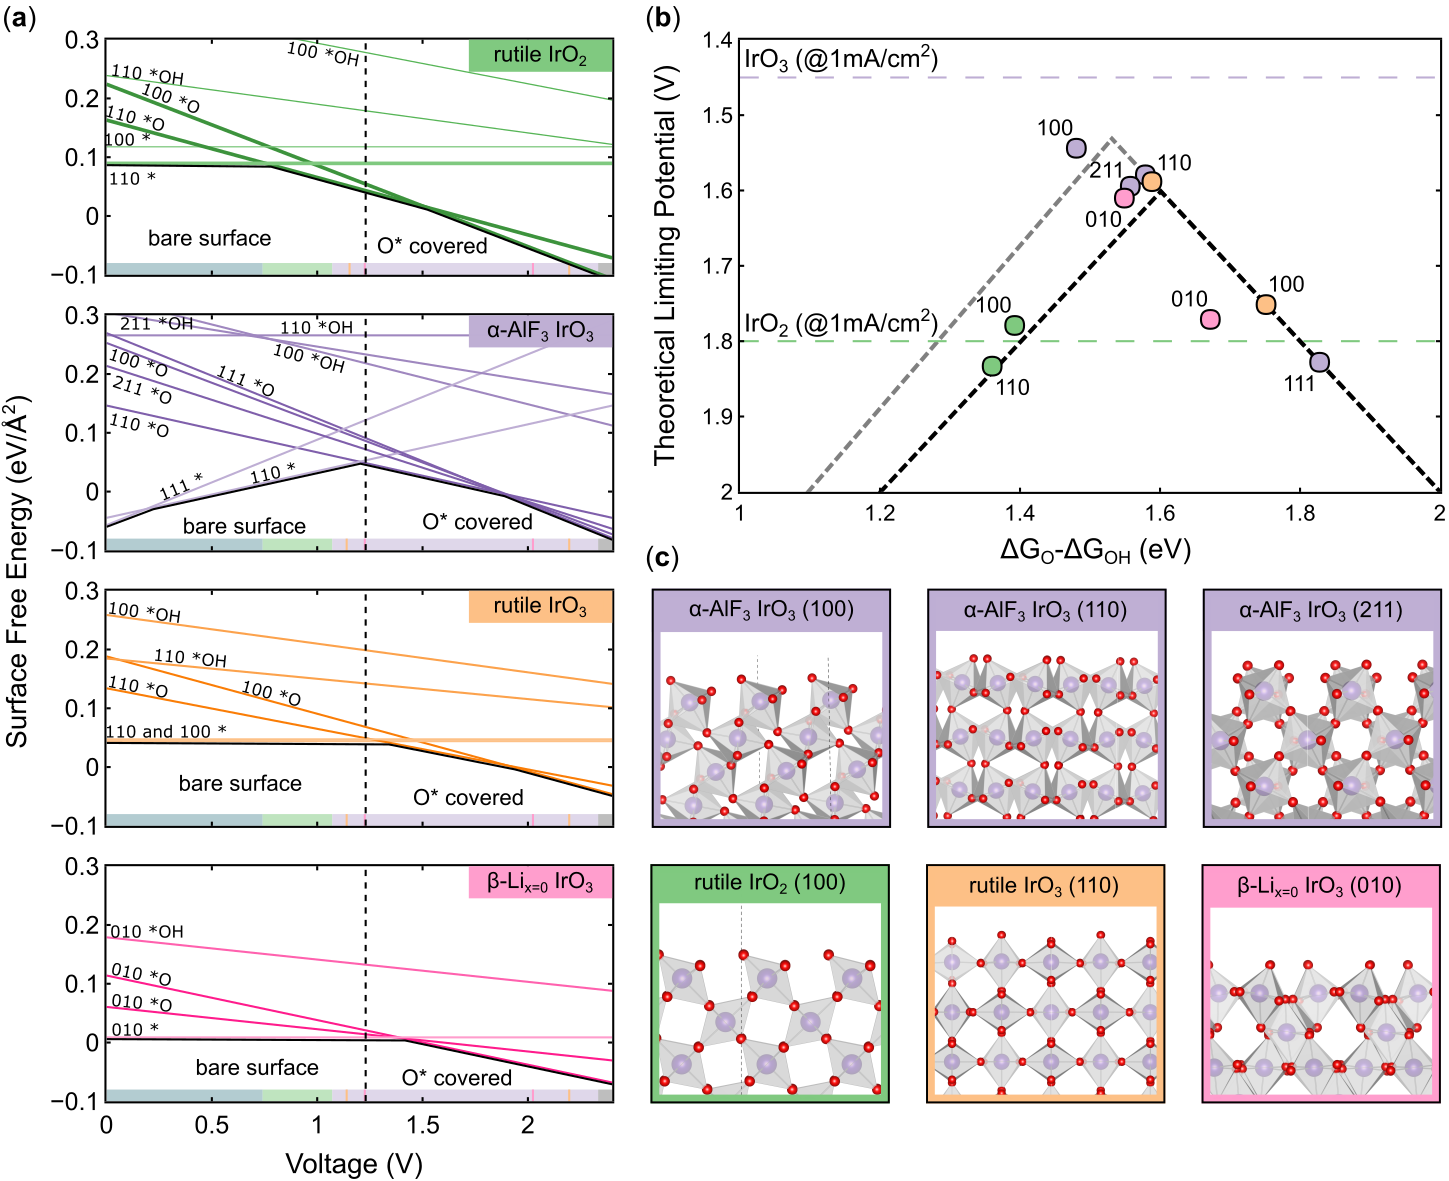
\includegraphics
{02_figures/oer_activity_stability/00_master__oer-volc_surf-pourb_struct__main_v3__200dpi__outplot.png}
% {02_figures/oer_activity_stability/00_master_plot__oer-volc_surf-pourb_struct__main_v3__outplot.pdf}
}
\caption{\label{fig:oer_volcano}
Summary of OER results for the four bulk structures of IrOx considered: rutile-IrO2 (green), $\alpha$-IrO3 (purple), rutile-IrO3 (orange), and b-IrO3 (pink).
(a) Surface energy Pourbaix diagrams for each structure, with the surface energy of various facets and coverages shown as a function of applied potential.
The bulk Pourbaix diagram's bounds of stability at pH 0 are superimposed at the bottom of each subplot.
(b) OER activity volcano for IrOx systems considered.
Circles designate oxygen covered surfaces while triangles designate hydroxyl (*OH) terminated surfaces (relevant surface terminations were found via surface Pourbaix analyses.
Surface energies at standard conditions (pH and V = 0) are reflected in the border color for each data point, where black indicates a low energy surface termination and white indicates more unstable surfaces.  % Currently not implemented as this
% The color range goes from x to y.
(c) Select surface structures for IrOx systems considered herin.
}
\end{figure}
% __|

% ################################# Paragraph #################################
% Surface Energy Pourbaix Analysis
To determine the most likely experimentally abundant surface facets and surface coverages, a surface energy Pourbaix diagram was constructed (TEMP).  % COMBAK Insert correct reference
See (SI for surface energy/Pourbaix part) for the method used to calculate surface energies.
% COMBAK
% __|

% | - OER Intermediate Scaling
\subsubsection{c. OER Intermediate Scaling}

% ################################# Paragraph #################################
Write stuff

% | - Figure | OER Scaling Relations
\begin{figure}
\centering
\makebox[\textwidth][c]{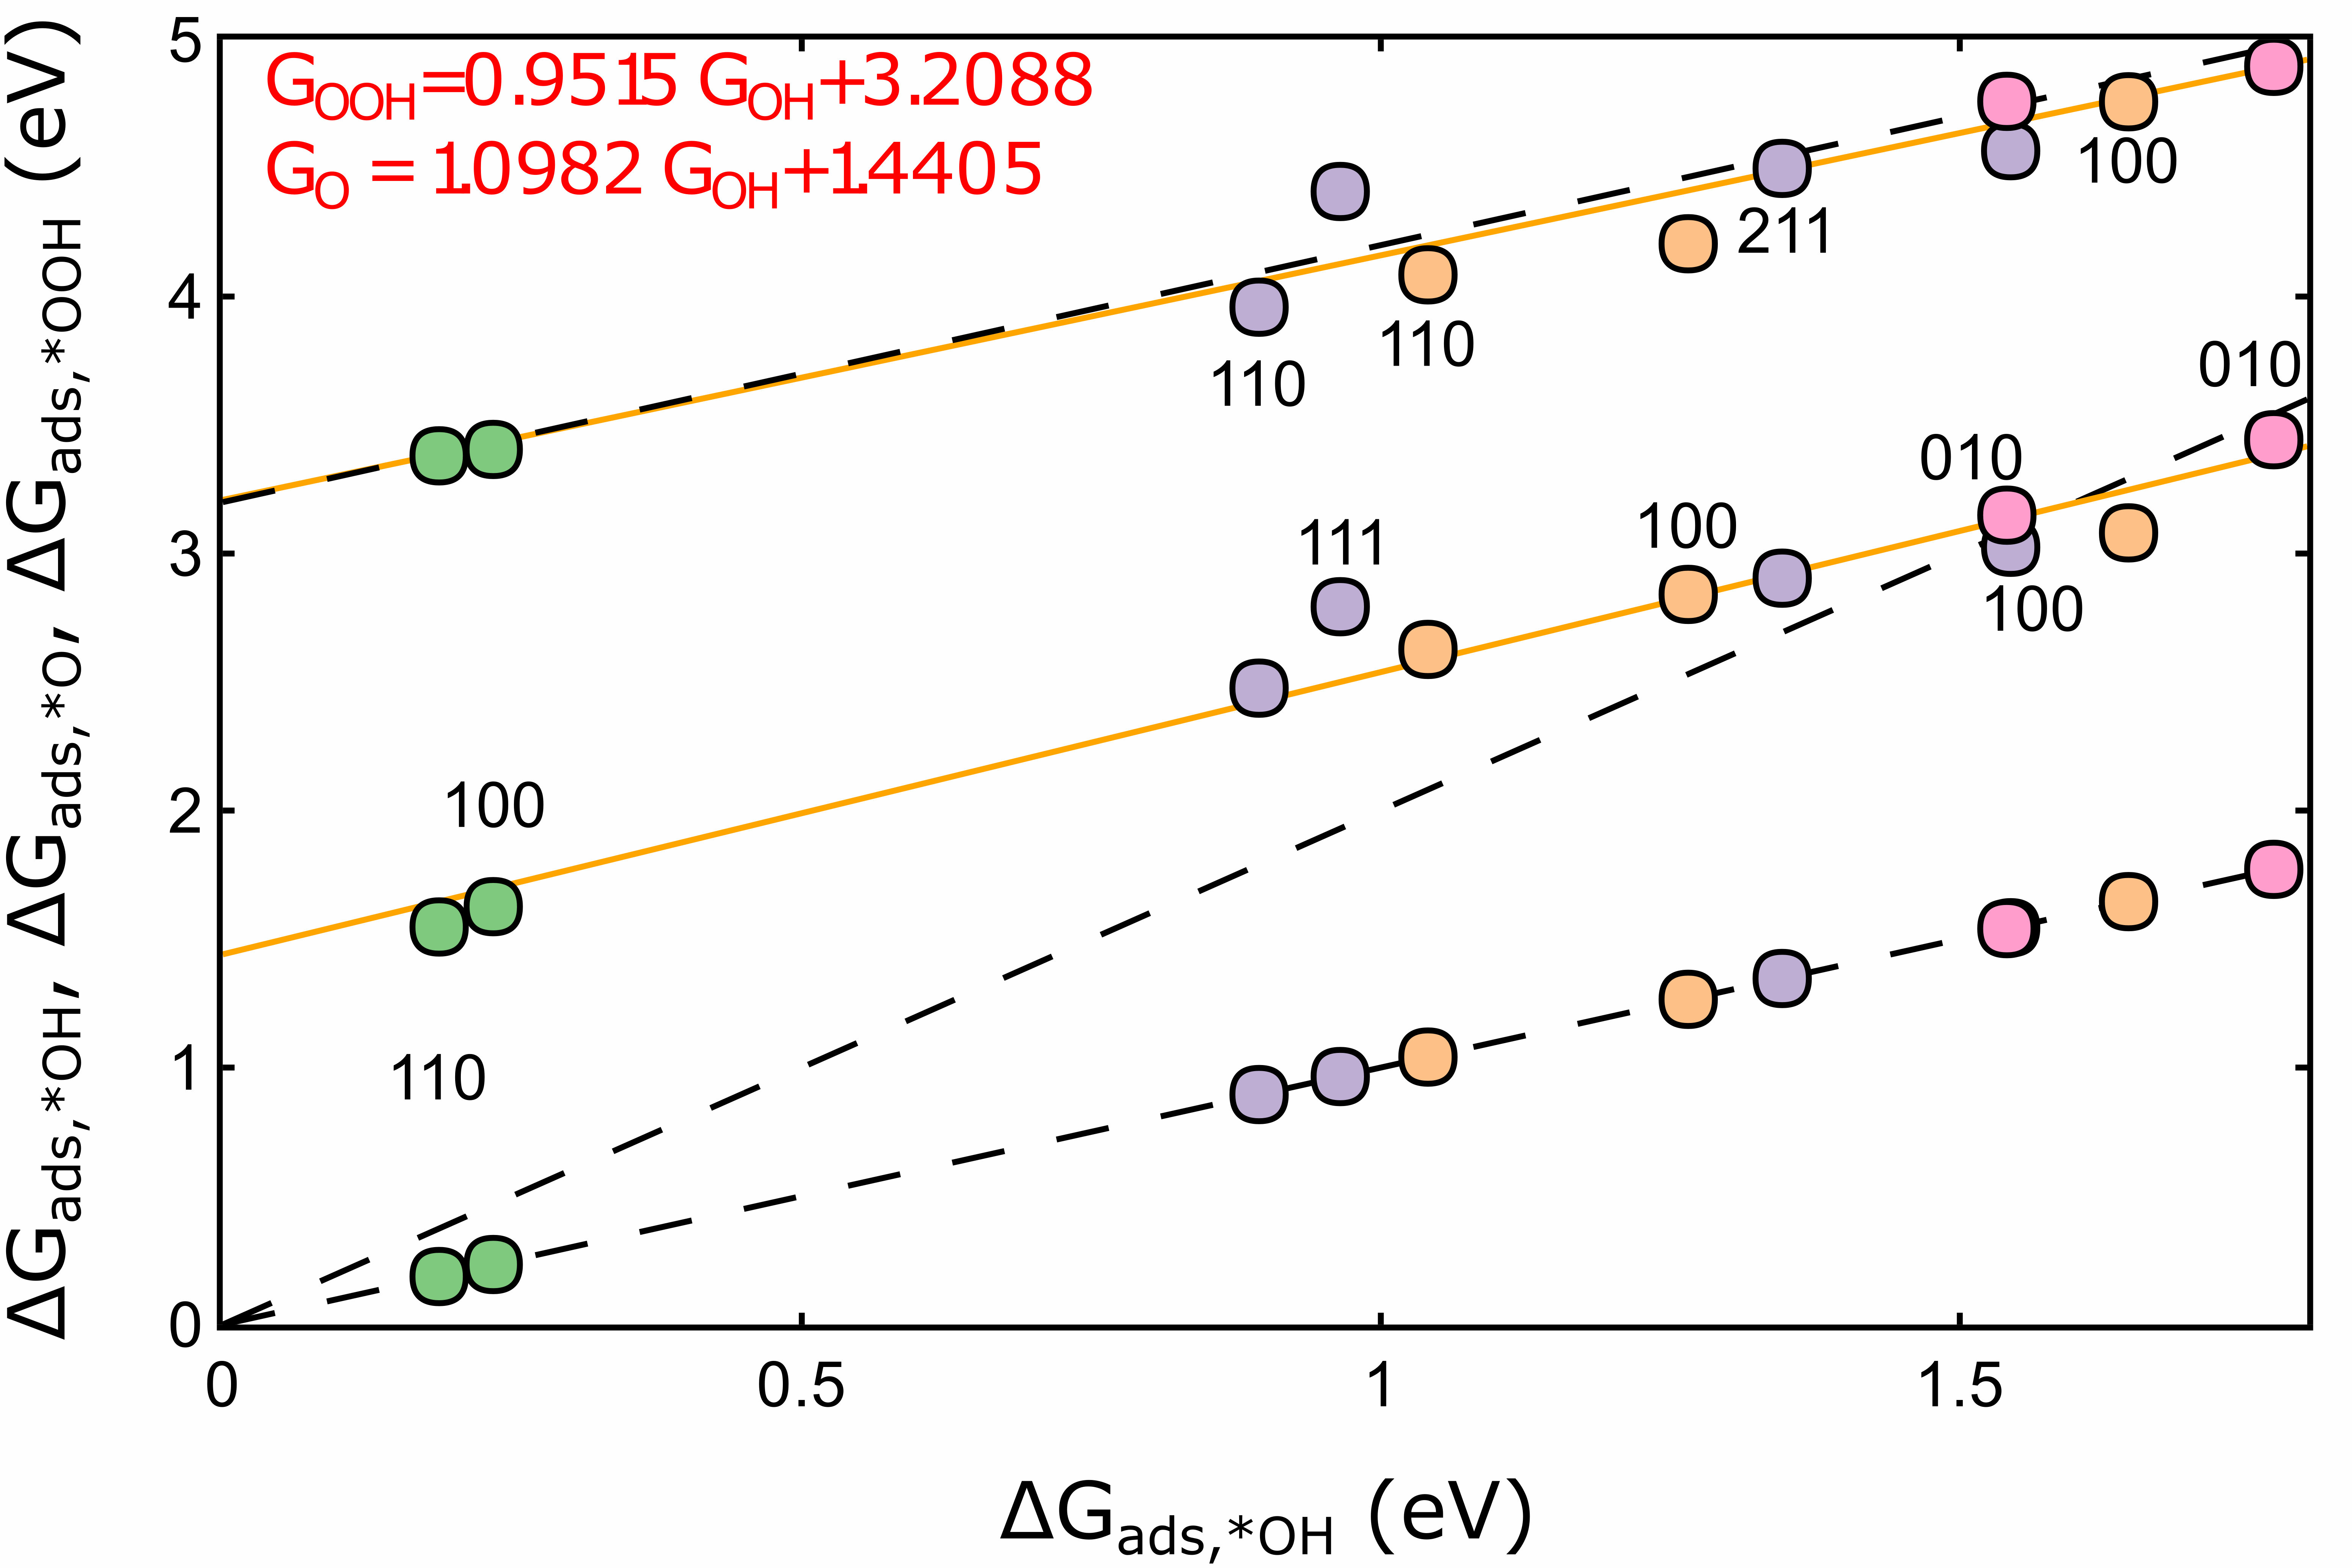
\includegraphics
{02_figures/oer_activity_stability/00_master__oer_scaling__main_v0__outplot2.png}
% {02_figures/oer_activity_stability/pl_scaling_relations_tmp.pdf}
}
\caption{\label{fig:scaling_relations}
Scaling relationship between DG of adsorption of the intermediate species of the OER using dG*OH as a descriptor.
DG*OOH, DG*O, and DG*OH are plotted on the y-axis.
}
\end{figure}
% __|

% __|
